\documentclass[mgr,oneside]{mgr}
\usepackage[polish]{babel}
\usepackage[utf8]{inputenc}
\usepackage{polski}
\usepackage[hidelinks]{hyperref}
\usepackage{graphicx}
\usepackage{listings}
\usepackage{color}
\frenchspacing
\linespread{1.3}
\usepackage{indentfirst}
\usepackage{caption}

\definecolor{mygreen}{rgb}{0,0.6,0}
\definecolor{mygray}{rgb}{0.5,0.5,0.5}
\definecolor{mymauve}{rgb}{0.58,0,0.82}

\lstset{
	backgroundcolor=\color{white},   % choose the background color
	basicstyle=\footnotesize,        % size of fonts used for the code
	breaklines=true,                 % automatic line breaking only at whitespace
	frame=single,
	commentstyle=\color{mygreen},    % comment style
	escapeinside={\%*}{*)},          % if you want to add LaTeX within your code
	keywordstyle=\color{blue},       % keyword style
	stringstyle=\color{mymauve},     % string literal style
}

\author{Marcin Mantke}
\title{Analiza porównawcza popularnych frameworków webowych.}
\engtitle{Comparative analysis of most popular web frameworks.}
\supervisor{dr inż. Roman Ptak}
\field{Informatyka (INF)}
\specialisation{Inżynieria systemów informatycznych (INS)}
\date{2017}

\begin{document}
\maketitle
\tableofcontents
% dodać rozdział z~wstępem teoretycznym, teoria do metod porównywania (5 rozdzial)
\chapter{Wstęp}
\section{Ogólny opis pracy}
W momencie pisania pracy istnieje niezliczona ilość frameworków webowych. Prawie codziennie, dla samego języka JavaScript, powstaje jeden nowy (micro) framework. Przyczyn takiego stanu rzeczy jest kilka. Po pierwsze, problemy, z~jakimi spotykają się programiści są bardzo zróżnicowane oraz skomplikowane. Wynika to z~nacisku biznesu, czyli klientów, na to, aby nowo powstały proukt był innowacyjny. Programista oczywiście posiada narzędzia, które powinny być wystarczające do rozwiązania powierzonego mu problemu, jednakże niekiedy korzystanie z~narzuconych przez framework rozwiązań wręcz utrudnia wykonanie powierzonej pracy. Z~tego powodu powstają nowe frameworki, które udostępniają zestaw narzędzi ukierunkowany pod rozwiązanie nowego, konkretnego problemu. Druga przyczyna jest w~pewien sposób powiązana z~pierwszą. Jest to stworzenie frameworku nie w~odpowiedzi na potrzebę, ale wygenerowanie potrzeby poprzez stworzenie frameworku, który ułatwia rozwiązanie przykładowego problemu. Kolejnym powodem jest próba odchudzenia istniejących frameworków. Przykładem może być Ruby~on~Rails, który jest frameworkiem kompletnym, ale niekiedy posiadającym zbyt dużo wbudowanych funkcji, z~których trudno jest zrezygnować, a~które w~danym projekcie nie zostaną wykorzystane. Zwiększa to rozmiar oraz złożoność projektu, co oczywiście jest niekorzystne.

Ilość dostępnych frameworków pokazuje jak ważnym elementem stały się one dla programistów. Niestety, tak dynamiczny rozwój rozwiązań tego typu powoduje spory problem jeśli chodzi o~wybór technologii. Ninejsza praca ma na celu zaprezentowanie wybranych frameworków webowych oraz dokonanie porównania ich funkcjonalności oraz wydajności. Analiza porównawcza ma na celu wyszczególnienie cech frameworków, na które programista powinien zwrócić szczególną uwagę przy doborze frameworku.

Jako że framework dodaje do aplikacji pewną warstwę abstrakcji, czyli kod, naturalny jest narzut wydajnościowy na aplikację. z~tego powodu, poza różnymi cechami odnośnie budowy i~dostarczanych funkcjonalności, frameworki różnią się również wydajnością.

\section{Cel pracy}

\section{Wymagania}
\section{Zarys koncepcji}

\chapter{Przedstawienie omawianych technologii}
\section{Historia i~rozwój technologii webowych}
Od lat 90 XX wieku świat obserwuje bardzo dynamiczny rozwój technologii związanych z~Internetem. Począwszy od roku 1991, kiedy to naukowcy z~instytu badawczego \textbf{CERN} (ang. \textit{European Organization for Nuclear Research}) opracowali standard WWW, przed programiastami zaczęła się otwierać nowa gałąź tworzenia aplikacji, którą są aplikacje internetowe. Początkowo aplikacje te były jedynie statycznymi stronami WWW, na których znajdował się jedynie tekst. Wprowadzenie kaskadowych arkuszy styli (\emph{CSS}) w~roku 1996 sprawiło, że strony internetowe przybrały graficzną formę. Rok 1997 przyniósł obsługę języka \emph{JavaScript} w~przeglądarkach internetowych. Oznaczało to, że strony internetowe, poza statycznymi elementami, zyskały elementy dynamiczne, np. reagujące na akcje użytkownika.

Wraz ze wzrostem dostępu ludzi do Internetu rozwijały się technologie odpowiedzialne za strony internetowe. Za punkt początkowy istnienia nie stron, a~aplikacji internetowych, można przyjać rok 1997 i~powstanie języka \emph{PHP}. Był to pierwszy interpretowany skryptowy język programowania, który służył do budowania aplikacji internetowych działających w~czasie rzeczywistym. Wraz z~rozwojem języka PHP oraz innych, podobnych mu języków, np. \emph{Python} i~\emph{Ruby}, zmienił się sposób budowania aplikacji. Programiści zaczęli rezygnować ze standardowych klientów w~postaci aplikacji desktopowych i~przechodzili na tzw. cienkich klientów (ang. \textit{thin client}). Trend ten przyspiesza rozwój oraz różnorodność aplikacji serwerowych posiadających interfejs graficzny w~formie strony internetowej, które nazywane są aplikacjami internetowymi \cite{historia}.

\section{Aplikacja internetowa}
Aplikacja internetowa (webowa) jest aplikacją znajdującą się nie na komputerze użytkownika, lecz na ogólnodostępnym serwerze. Komunikacja pomiędzy, niekiedy rozproszonymi, elementami aplikacji odbywa się poprzez sieć komputerową. Aplikacja webowa swój interfejs graficzny poprzez przeglądarkę internetową bądź np. aplikację mobilną.

\section{Framework webowy} % moduły i~biblioteki, np do połączenia z~bazą danych
Aby ułatwić korzystanie z~coraz liczniejszych technologii wykorzystywanych w~tworzeniu aplikacji internetowych, powstały narzędzia nazywane frameworkami webowymi. Framework jest uniwersalnym środowiskiem programistycznym, które dostarcza niezbędne narzędzia wymagane do stworzenia aplikacji internetowej w~wybranym języku programowania \cite{framework}. Każdy z~frameworków dostarcza pewną abstrakcję, która znajduje się wokół kodu napisanego przez programistę. Przykładem takiej abstrakcji jest system mapowania ścieżki podstrony (np. \textit{/users/3}) na konkretną akcję w~aplikacji (zwykle akcja \emph{SHOW} dla kontrolera \emph{Users}), czyli \emph{routing}. Twórcy frameworków zauważyli, że w~każdej aplikacji webowej są stosowane te same typy rozwiązań, więc w~wielu przypadkach wprowadzili dane rozwiązania jako integralne części frameworków. W~efekcie programiści mogą korzystać z~gotowych, dogłębnie przetestowanych rozwiązań, które znajdują się w~90\% aplikacji webowych.

\chapter{Przegląd wybranych rozwiązań}
\section{Ruby on Rails}
Ruby on Rails jest open source'owym frameworkiem webowym. Został stworzony w~głównej mierze przez duńskiego programistę Davida Heinemeiera Hanssona. Pierwsza wersja RoR ukazała się w~lipcu 2004 roku. Fakt ten pokazuje, że jest to już dojrzały framework, z~ugruntowaną pozycją na rynku. Potwierdzeniem tej pozycji jest liczne wsparcie społeczności. Rails'y zostały stworzone przez ponad 4,5 tysiąca osób, istnieje ok. 132 tysiące ogólnodostępnych paczek, które rozszerzają funkcjonalność tego frameworku. Ruby on Rails domyślnie korzysta z~architektury MVC, czyli \emph{Model - View - Controller}.

\subsection{Doktryna Ruby on Rails}
Tworzeniu i~rozwojowi Ruby on Rails towarzyszy kilka podstawowych zasad. Jedne istnieją od początku, inne ewoluowały na przestrzeni lat. Spisane są one w~\emph{The Rails Doctrine} \cite{rails_doctrine}. Na potrzeby pracy zostaną omówione najważniejsze z nich.

\subsubsection{Optimize for programmer happiness}
Pierwsza reguła odnosi się mocno do języka, z~którego wywodzą się Rails'y. Sam fakt umieszczenia nazwy języka Ruby w~nazwie frameworku pokazuje jak ważny jest on dla całego projektu. Motywacją stworzenia języka Ruby była chęć dostarczenia programistom radości z~pisania kodu. w~momencie powstawania Ruby'ego, większość popularnych wtedy języków programowania narzucało sposób pisania bądź stosowało liczne ograniczenia w~sposobie pisania kodu. Ruby stał w~opozycji do tych zasad, dając programistom pełną dowolność w~sposobie tworzenia kodu.

Jako przykład owego ,,uwolnienia'' programisty podawana jest \emph{Zasada Najmniejszego Zaskoczenia} (ang. The Principle of Least Surprise).
\begin{lstlisting}[caption={Wyjście z~interpretera Ruby'ego.},language=Ruby]
$ irb
irb(main):001:0> exit
$ irb
irb(main):001:0> quit
\end{lstlisting}

\begin{lstlisting}[caption={Wyjście z~interpretera Python'a.},language=Python]
$ python
>>> exit
Use exit() or Ctrl-D (i.e. EOF) to exit
\end{lstlisting}
Ruby zaakceptuje oba polecenia opuszczenia interpretera. Python natomiast, pomimo odczytania intencji programisty (wyświetlenie instrukcji), opuści interpreter jedynie po wpisaniu komendy \emph{exit()} lub po użyciu kombinacji klawiszy \emph{Ctrl-D}, co oczywiście nie jest zgodne z~oczekiwaniami programisty.

Wzorując się na zasadach, na których powstawał Ruby, Rails'y również miały umilać życie programistom. Jako przykład jest podawana klasa \emph{Inflector}. Zapisane są w~niej reguły oraz wyjątki od reguł w~języku angielskim, które umożliwiają mapowanie klasy \emph{Comment} na tabelę \emph{Comments}, \emph{Person} na \emph{People} itp. Kolejnym przykładem może być dodatek do Ruby'owej klasy \emph{Array}, który poza dostępnym w~Rubym pierwszym elementem tablicy, umożliwia dostęp do kolejnych czterech elementów tablicy, poprzez wyrażenia \emph{Array\#second,~Array\#third} itd.

Oczywiście nie są to kluczowe cechy frameworku, ale stanowczo zaznaczają ważkość celu, którym jest przede wszystkim sprawianie radości z~tworzenia oprogramowania.

\subsubsection{Convention over Configuration}
Twórcy Ruby on Rails starają się kłaść mocny nacisk na prostotę używania ich narzędzia. Zamiast zrzucać na programistów ciągłe podejmowanie decyzji w~kwestiach mało istotnych, jak na przykład format klucza obcego w~bazie danych, Rails'y narzucają konwencję nazewnictwa. Oczywiście jest możliwość konfiguracji narzuconych przez framework konwencji, lecz jest to raczej rzadko spotykane, a~wręcz niewskazane. Zasada ta, poza zdjęciem odpowiedzialności za część decyzji z~barków programisty, przynosi również inne korzyści.

Dzięki ,,domyślnej'' konwencji, możliwe jest stworzenie głębszej abstrakcji, na której operuje framework. Przykładem może być zastosowanie wcześniej wymienionej klasy \emph{Inflector}. Jeśli możliwe jest zmapowanie klasy \emph{Person} na tabelę \emph{People}, to możliwe jest również zmapowanie relacji \emph{has\_many: people} w~taki sposób, aby wykorzystywana była klasa \textit{Person}. Jest to o~tyle wygodne rozwiązanie, że nawet pomimo posiadania wiedzy na temat tworzenia relacji w~bazie danych oraz sposobu odzwierciedlania ich w~kodzie aplikacji, programista nie musi przejmować się tworzeniem lub konfiguracją tej części aplikacji.

Kolejną zaletą jest znaczące obniżenie progu wejścia dla początkujących programistów. Takim osobom dużo łatwiej jest poznawać framework stopniowo. Począwszy od poziomu, gdzie wszystko automatycznie działa, lecz nie wiadomo dlaczego, aż do momentu gdzie nadal wszystko automatycznie działa, ale bardzo dobrze wiadomo dlaczego. Znaczna część mechanizmów stosowanych we frameworkach webowych \emph{de facto} nie wymaga niestandardowej konfiguracji, nawet jeśli programista posiada szeroką wiedzę w~danej dziedzinie. Przekładanie konfiguracji ponad konwencję wymaga od programisty sporego wysiłku, aby rozpocząć pracę z~frameworkiem, co w przypadku poznawania nowych technologii stanowczo nie jest zachęcające.

Zasada ta bywa jednak zgubna. Jest tak z~powodu błędnego przekonania, że skoro od samego początku wszystkie elementy aplikacji można wygenerować, i~od samego początku wszystko działa, to programista nie musi mieć wiedzy na temat tego, co robi. W~przypadku bardzo podstawowych zastosowań wiedza programisty rzeczywiście nie musi być szeroka, natomiast bardzo problematyczne jest w~takim przypadku wykonanie części aplikacji, która jest niestandardowa bądź niemożliwa do wygenerowania.

\subsubsection{The menu is omakase}
Rzadko kiedy framework jest monolitem, który nie składa się z~modułów. Częściej framework jest zbiorem mniejszych frameworków lub bibliotek, które współpracują ze sobą. Bardzo często wybór owych narzędzi leży w~pełni po stronie programisty. Jako analogię takiego wyboru, w \emph{The Ruby on Rails Doctrine} podawany jest problem wyboru dania z~menu w~restauracji, którą odwiedzamy po raz pierwszy. Jeśli zdamy się na wybór szefa kuchni, możemy założyć że jedzenie będzie dobre, nie wiedząc jeszcze co ,,dobre'' będzie oznaczać \cite{rails_doctrine}.

Ruby on Rails rozwiązuje ten problem poprzez dostarczenie zestawu narzędzi, z~których programista może korzystać. Zasada działania jest tutaj bardzo zbliżona do reguły \emph{Convention over Configuration}, lecz operuje na wyższym poziomie abstrakcji. Programista dostaje zestaw domyślnych narzędzi, z~którego może od samego początku korzystać, bez potrzeby podejmowania decyzji odnośnie wyboru frameworków i~bibliotek. Ma on natomiast możliwość zamiany domyślnie wybranych narzędzi na inne, jeśli widzi taką potrzebę.

Zasada ta niesie za sobą korzyści w~sferze rozwoju frameworku. Jest tak, ponieważ programiści, używając tych samych narzędzi, są w~stanie bardziej dopracować owe narzędzia. Częstym problemem jest nie fakt jak działa dany framework bądź biblioteka w~izolacji, lecz jak działa razem z~innymi modułami. Jeśli wielu programistów napotyka te same błędy w~integracji poszczególnych składowych frameworku, to dużo łatwiej jest twórcom takie błędy poprawić bądź usprawnić połączenie tych modułów.

\subsubsection{No one paradigm}
Twórcy frameworka Ruby on Rails są przekonani, że nie istnieje jedno idealne rozwiązanie. Często do jednego celu można dojść różnymi drogami. Z~tego też powodu, pomimo wyboru architektury MVC, Railsy są bardzo elastyczne jeśli chodzi o~dostosowanie się do innych modeli projektowych. Domyślnie RoR nie posiada wbudowanych \textit{Serwisów} bądź \textit{Prezenterów}, lecz framework jest zbudowany w~taki sposób, aby użycie większości wzorców projektowych było bezproblemowe.

Przystosowanie frameworku do korzystania z~różnych wzorców projektowych poniekąd wymusza na programistach znajomość większej ilości owych wzorców. Jako, że Ruby jest bardzo elastycznym językiem jeśli chodzi o~paradygmaty programowania, ponieważ możliwe jest pisanie funkcyjne, Railsy również wspierają owe podejście. Od programisty zależy, czy z~takiej możliwości skorzysta. Wprowadzenie takiej uniwersalności niestety niesie za sobą spory nakład pracy ze strony twórców.

\subsection{Pozostałe cechy}
Poza cechami wymienionymi w \textit{The Ruby on Rails Doctrine}, Ruby on Rails kładzie mocny nacisk na inne aspekty. Są to m.in. kwestie takie, jak przestrzeganie reguły \textit{DRY} (ang. \textit{Don't Repeat Yourself}) bądź też wsparcie dla dodatkowych bibliotek rozszerzających funkcjonalność frameworku.

\subsubsection{Don't Repeat Yourself}
Reguła \textit{DRY} mówi o tym, aby, jak sama nazwa wskazuje, nie powtarzać kodu. Każde powtórzenie logiki biznesowej może być rozwiązane poprzez dodanie warstwy abstrakcji. Natomiast duplikację procesów można rozwiązać poprzez ich automatyzację \cite{dry}. Poprzez stosowanie tej reguły, kod aplikacji jest wyraźnie mniejszy, ale przede wszystkim jest on bardziej odporny na błędy i łatwiejszy w utrzymaniu. Jeśli w~powtarzającym się fragmencie kodu zostanie popełniony błąd, dzięki zastosowaniu reguły DRY, zmianę trzeba wprowadzić tylko w~jednym miejscu, a~nie w~każdym wystąpieniu powtarzającej się funkcji.

Ruby on Rails wspiera używanie tej reguły poprzez wbudowane w framework elementy, takie jak \textit{Helpery}, \textit{Concerny} lub \textit{Partiale}. Umożliwiają one wspóldzielenie kodu i używanie ich w każdej z warstw aplikacji.

\subsubsection{Biblioteki}
Biblioteki tworzone przez społeczność nie są bezpośrednio elementem frameworku, ale samego języka Ruby. Ich nazwa to \textit{gem'y}. Rails'y natomiast mają domyślnie dołączony menedżer bibliotek/pakietów - \textit{bundler}.

\begin{figure}[h]
  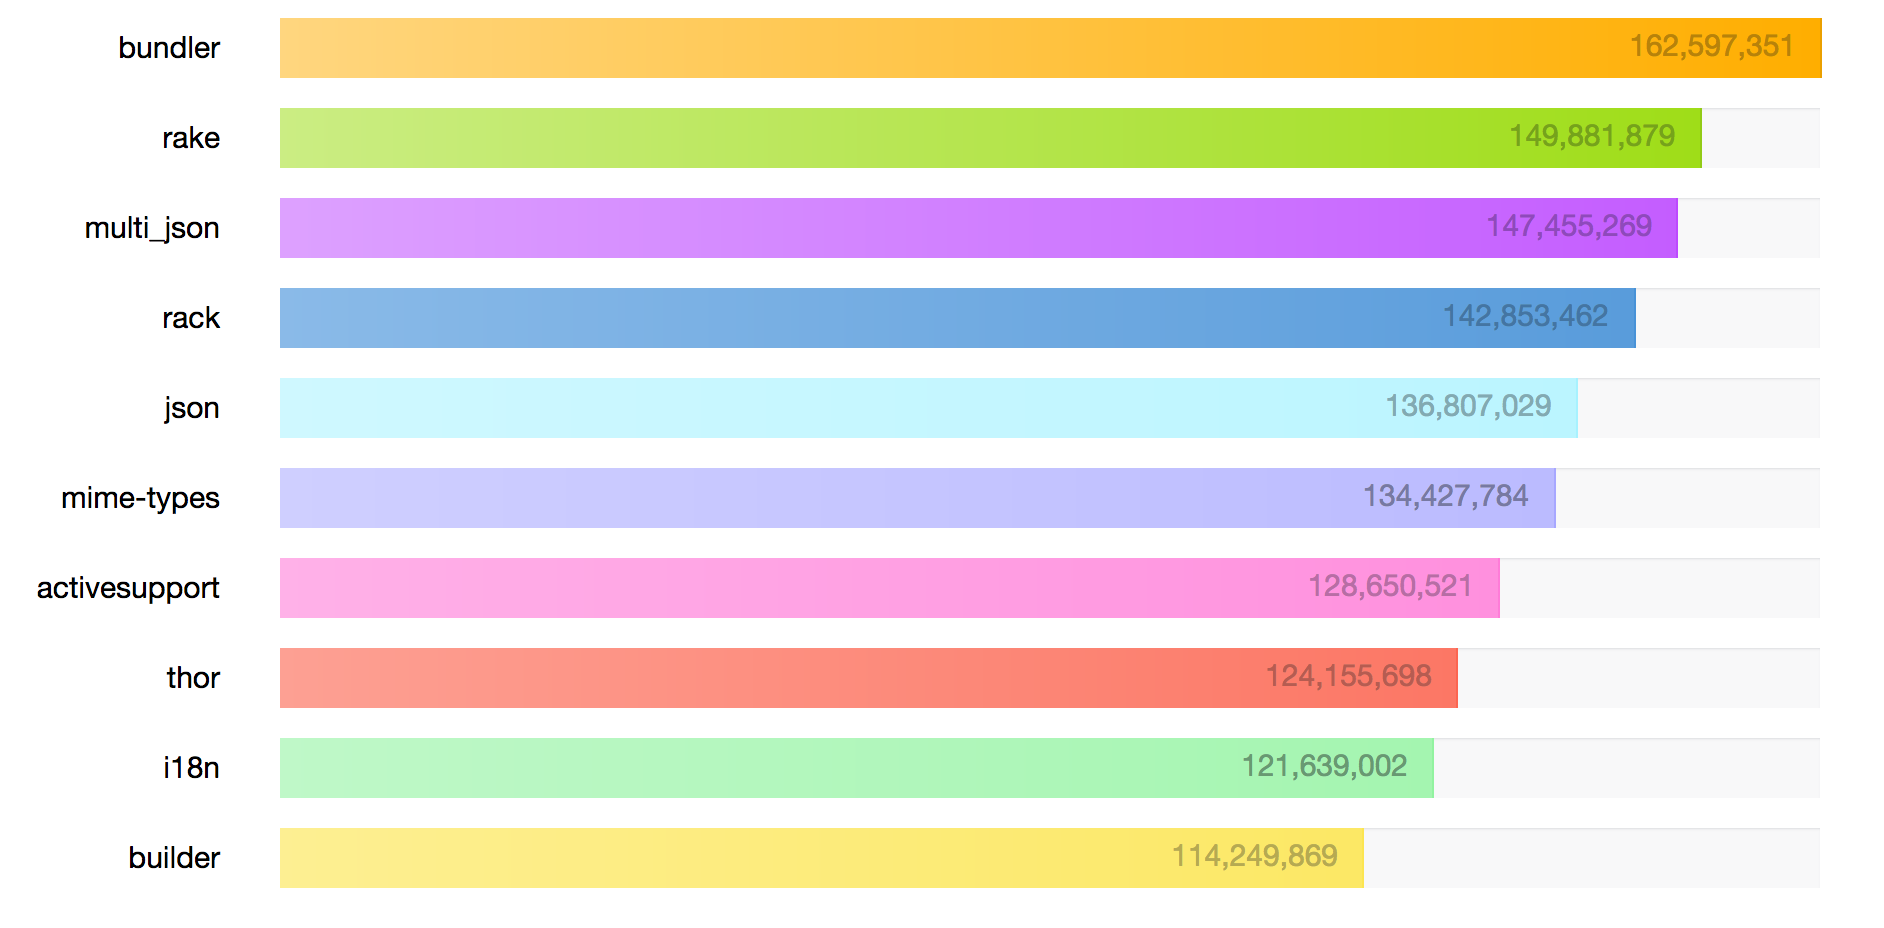
\includegraphics[width=\linewidth]{images/bundler_stats}
  \caption{Statystyki pobrań menedżera pakietów bundler.}
  \label{fig:bundler_stats}
\end{figure}

Jak widać, \textit{bundler} jest najczęściej pobieranym \textit{gem'em} spośród wszystkich, z ilością pobrań przekraczającą 162,5 miliona. Ogromny wpływ na taki wynik mają oczywiście Rails'y. Strona \url{https://rubygems.org/}, która jest źródłem większości bibliotek, w statystykach podaje, że dostępnych jest ponad 131,600 paczek. Pokazuje to jak ważną częścią dla twórców Ruby on Rails i całej społeczności jest możliwość tworzenia rozszerzeń oraz ich dostępność.

\section{Phoenix} % https://media.pragprog.com/titles/phoenix/intro.pdf   http://www.phoenixframework.org/docs/resources
\section{Express}

\chapter{Analiza porównawcza}
\section{Opisowe porównanie charakterystyki wybranych frameworków}
\subsection{Ruby on Rails vs Phoenix}
\subsection{Ruby on Rails vs Express}
\subsection{Phoenix vs Express}
\section{Subiektywna ocena}

\chapter{Implementacja}
\section{Ruby on Rails}
\section{Phoenix}
\section{Express}

\chapter{Projekt komputerowego środowiska eksperymentalnego}
\section{Plan prowadzenia eksperymentów}

\section{Wykorzystane narzędzia}
\subsection{Nginx}
\subsection{Docker}
\section{Benchmarki}
% https://www.sitepoint.com/tools-testing-website-performance/
\subsection{Ruby}
% http://rubylearning.com/blog/2013/06/19/how-do-i-benchmark-ruby-code/
\subsection{Elixir}
% https://github.com/PragTob/benchee
\subsection{JavaScript}
% https://benchmarkjs.com/

\chapter{Analiza wydajnościowa}
\label{cha:analiza_wydajnosciowa}
\section{Metody mierzenia wydajności aplikacji internetowych}
\section{Wyniki badań}

\chapter{Podsumowanie}
\renewcommand\bibname{Literatura}
\begin{thebibliography}{inteligencja}
	\addcontentsline{toc}{chapter}{Literatura}

  \bibitem{historia}
  \emph{Historia Internetu}, dostęp pod adresem: \url{https://pl.wikipedia.org/wiki/Historia_Internetu}, aktualne na dzień 1.04.2017r.

  \bibitem{framework}
  \emph{Software framework}, dostęp pod adresem: \url{https://en.wikipedia.org/wiki/Software_framework}, aktualne na dzień 1.04.2017r.

	\bibitem{rails_guide}
	\emph{Ruby on Rails Guides}, dostęp pod adresem: \url{http://guides.rubyonrails.org/},\\ aktualne na dzień 14.06.2017r.

  \bibitem{rails_doctrine}
  \emph{Ruby on Rails Doctrine}, dostęp pod adresem: \url{http://rubyonrails.org/doctrine/}, aktualne na dzień 1.05.2017r.

  \bibitem{phoenix_doctrine}
  McCord R., Tate B., Valim J., \emph{Programming Phoenix}, The Pragmatic Programmers LLC, 2016
	\bibitem{cleancode}
	Martin, R. \emph{Czysty kod. Podręcznik dobrego programisty}, Gliwice, Wydawnictwo Helion 2010

  \bibitem{benchmarking_tools}
  Diwan, A. \emph{Tools for Testing Website Performance}, dostęp pod adresem: \url{https://www.sitepoint.com/tools-testing-website-performance/}, \\ aktualne na dzień 18.03.2017r.

  \bibitem{dry}
  \emph{Don't Repeat Yourself}, dostęp pod adresem: \url{http://deviq.com/don-t-repeat-yourself/}, aktualne na dzień 3.05.2017r.

\end{thebibliography}
\end{document}
